\section{What finite information cannot decide}\label{ch:finite}

Every computation in this book is finite: a finite window, finitely many resolutions, finitely many derivatives or matrix blocks. Theorem~\ref{thm:ch13:perturb} replaces two close zeros of $\xi$ on the line by a quadruple off it \cite[Chapter 11]{P26} and obtains an entire function whose heat trace passes the finite tests of Section~\ref{ch:heat}. Below height $2000$ the order at which its derivative signs first fail can be computed, and it grows roughly like the square of the height. Section~\ref{sec:ch13:visibility} records what each finite test of the book establishes and what it cannot exclude; the sharpest case is positivity of $\rho_\varepsilon$ at one resolution, which can miss zeros far from the line. Finally, a finite computation can refute a sufficient condition for RH: one certified zero of an explicit function closes the Bernstein Pick route through the moments of the P\'olya density.

\subsection{A perturbation that passes the finite tests of the heat trace}\label{sec:ch13:perturb}

\begin{theorem}[{\cite[Theorem D]{P17}}]\label{thm:ch13:perturb}
\textup{(a)} There are ordinates $1000<A<B\le2000$ of zeros on the critical line, with $B-A\le2$, such that, with $g=(A+B)/2$ and $w=\frac14+ig$,
\[
F(s)=\frac{\xi(\frac12+s)}{\xi(\frac12)}\,\frac{(1-s^2/w^2)(1-s^2/\bar w^2)}{(1+s^2/A^2)(1+s^2/B^2)}
\]
is an even entire function with the order, type and reflection symmetry of $\xi(\frac12+s)$ and with four zeros off the critical line, and the following hold. The reciprocal clock $1/F(\sqrt u)$ is the Laplace transform of an infinitely divisible, self decomposable law, and its heat trace
\[
W_F(t)=W(t)+2\re e^{-at}-e^{-A^2t}-e^{-B^2t},\qquad a=-w^2=g^2-\tfrac1{16}-\tfrac{ig}2,
\]
which is $t$ times its L\'evy density, is strictly log convex. $W_F$ has the same small time expansion as $W$ through the constant term, and $1/F$ has the same nearest poles as the reciprocal Xi function.

\textup{(b)} Let $N\ge1$ and $R\ge T_N$, where $T_N=20000N\sqrt{1+\log N}$ as in Section~\ref{ch:heat}, and suppose that every zero of $\xi$ with ordinate in $(0,R+50]$ lies on the critical line. Then the pair can instead be chosen with $R<A\le B\le R+50$ and $B-A<2$ (if $A=B$, a multiple zero supplies both), so that $F$ keeps every property listed in (a) and the leading $N\times N$ Hankel blocks of $W_F$ remain positive definite at every $t>0$. If moreover $R\ge10^{12}$, the derivative signs of Theorem~\ref{thm:ch12:cm} are also preserved: $(-1)^kW_F^{(k)}(t)>0$ for every $t>0$ and every integer $0\le k\le10^{17}$. For every $N\le3\times10^7$ the verification to height $3\times10^{12}$ \cite{PT21} establishes the hypothesis on the zeros for $R=\max(T_N,10^{12})$, so that such an $F$ with both properties exists unconditionally.
\end{theorem}

The construction moves the zeros at heights $A$ and $B$, with their conjugates, to the quadruple $\frac12\pm\frac14\pm ig$. The heat trace changes by the oscillating term $W_F-W$, whose envelope is bounded as in Section~\ref{ch:heat} \cite[Proposition 11.1]{P17}, and at the heights of (b) this change is smaller than the margin by which each of its tests holds. The pair of (b), with the properties of (a) and the Hankel blocks, comes from \cite[Theorem 12.5]{P17}, the derivative signs from \cite[Proposition 12.7]{P17}, which holds for any pair of zeros on the line with $A>10^{12}$ and $B-A\le2$, and the unconditional range from \cite[Corollary 12.6]{P17}, since $T_{3\times10^7}+50<2.6\times10^{12}$. Figure~\ref{fig:ch13:perturb} shows the change for a pair in the range of (a), far below the heights that (b) requires; the pair it moves, near height $1977.22$, is the closest pair among the first $1700$ zeros, whether or not the spacings are normalised (Section~\ref{sec:ch15:spacings}).

\begin{figure}[htbp]
\centering
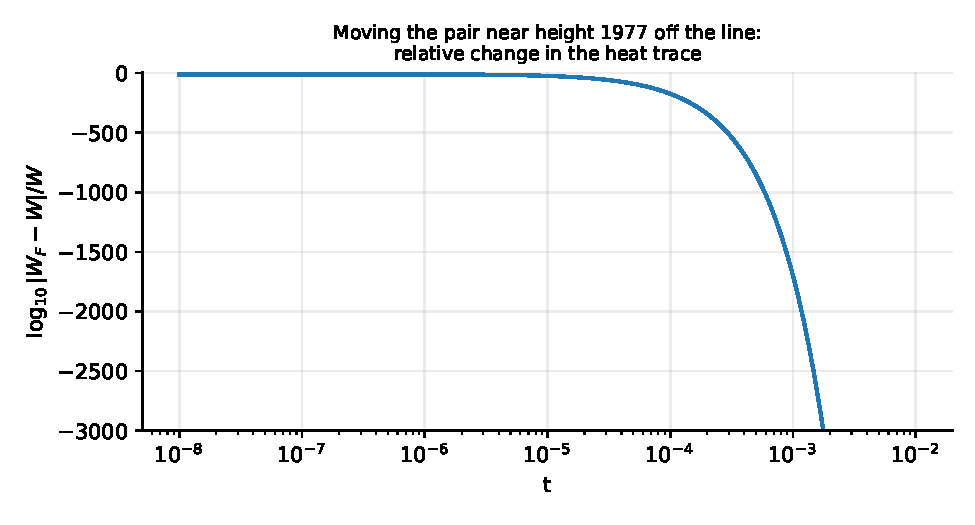
\includegraphics[width=0.72\textwidth]{fig/perturb.pdf}
\caption{Relative change $|W_F-W|/W$ of the heat trace, on a $\log_{10}$ scale, when the closest pair of zeros between heights $1000$ and $2000$ (near $1977.22$) is moved to distance $\frac14$ from the line, computed in forty digit arithmetic with $W$ replaced by its sum over the first $1700$ zeros. The change is at most $4\times10^{-11}$, near $t=7\times10^{-7}$, and falls below $10^{-1000}$ by $t=10^{-3}$. The sum over $1700$ zeros is smaller than $W$, by $1.3$ per cent at $t=7\times10^{-7}$ and by a factor of $5.4$ at $t=10^{-8}$, so the curve bounds the relative change from above; with $W$ from the explicit formula \eqref{eq:ch2:Warith} the maximum is $3.66\times10^{-11}$, at $t=7.2\times10^{-7}$.}
\label{fig:ch13:perturb}
\end{figure}

Not every finite test is passed. Below any height $T>B$ the argument count of $F$ equals that of $\xi$, since $F$ loses the zeros at heights $A$ and $B$ and gains two at height $g$, but these two are off the line, so $F$ has two zeros fewer on the line, counted with multiplicity; when $A<B$ and both zeros are simple, as for the pair of Figure~\ref{fig:ch13:perturb}, it has two sign changes fewer. Turing's comparison of the two counts, the first test of Table~\ref{tab:ch13:see}, then detects the perturbation once it passes height $B$, and the zero density identity at any height $T>g$ returns $\nu(\frac12+\varepsilon,T)\ge1$ for every $\varepsilon<\frac14$, whatever the multiplicities. Counting tests are local in height and find the perturbation once their window contains it, whereas a given finite set of heat trace tests, which involve all the zeros at once, misses it when it lies high enough.

The pair of Figure~\ref{fig:ch13:perturb} lies far below the heights of (b), and at its height the derivative signs of $F$ do fail at a finite order, which can be computed. On the ray $t=k/u^2$ the normalised value $e^{-f_0}c_k^F(t)$ of Proposition~\ref{prop:ch12:ray}, whose proof applies to $F$ because $F$ has at most one zero more than $\xi$ below any height, is a sum of positive terms, one for each zero on the line, the oscillating term of the quadruple and terms, negligible here, from any zeros off the line above $3\times10^{12}$, and only the zeros within a few units of $u$ matter. A scan over $u$ and over the orders, at every order up to $500$, then on a grid of ratio $1.002$ and at every order of the last grid interval, finds that the first order at which $c_k^F(t)<0$ for some $t>0$ is $k=6\,683\,655$, at $t=1.7113393$. The grid loses nothing, because $c_{k-1}^F(t)=\int_t^\infty c_k^F(s)\,ds$: if $c_k^F\ge0$ on $(0,\infty)$ then so is $c_{k-1}^F$, and the orders that fail are all those from the first one on. The negative value is certified in ball arithmetic, with explicit bounds for the zeros below $g-40$, which lie on the line, and for those above $g+40$, wherever the ones above $3\times10^{12}$ lie; the positivity at the lower orders is computed, not certified. Table~\ref{tab:ch13:first} repeats the computation for the closest pair of consecutive zeros in five other windows of height, and for the pair near $1977.22$ moved to distance $0.1$ instead of $\frac14$.

\begin{table}[htbp]
\centering\small\setlength{\tabcolsep}{4pt}
\begin{tabular}{rrrrrrr}
\toprule
window & zeros moved & $g$ & $\delta$ & $k^*$ & $t^*$ & $c_{k^*}^F(t^*)$, normalised\\
\midrule
$(100,200)$ & $71$, $72$ & $185.24$ & $\frac14$ & $40\,018$ & $1.18413$ & $-6.37\times10^{-7}$\\
$(200,400)$ & $186$, $187$ & $376.08$ & $\frac14$ & $219\,169$ & $1.54072$ & $-6.70\times10^{-8}$\\
$(400,700)$ & $363$, $364$ & $630.64$ & $\frac14$ & $624\,921$ & $1.576635$ & $-1.68\times10^{-7}$\\
$(700,1000)$ & $453$, $454$ & $750.81$ & $\frac14$ & $792\,746$ & $1.410725$ & $-9.26\times10^{-8}$\\
$(1000,1500)$ & $922$, $923$ & $1329.12$ & $\frac14$ & $4\,433\,220$ & $2.5121193$ & $-3.37\times10^{-8}$\\
$(1500,2000)$ & $1496$, $1497$ & $1977.22$ & $\frac14$ & $6\,683\,655$ & $1.7113393$ & $-7.12\times10^{-9}$\\
$(1500,2000)$ & $1496$, $1497$ & $1977.22$ & $0.1$ & $15\,722\,219$ & $4.0257254$ & $-6.71\times10^{-11}$\\
\bottomrule
\end{tabular}
\caption{The first failing order of the derivative signs when the closest pair of consecutive zeros in a window of height is moved to the quadruple $\frac12\pm\delta\pm ig$, $g$ the midpoint of the pair. $k^*$ is the least order at which $c_k^F(t)<0$ for some $t>0$, found by a scan of every order up to $500$, a grid of ratio $1.002$ above it and every order of the last grid interval (computed, not certified); $c_{k^*}^F(t^*)<0$ is certified in ball arithmetic. The last column is $c_{k^*}^F(t^*)$ divided by $(k^*/t^*)^{k^*}e^{-k^*}$, the value at $x=k^*/t^*$ of the weight $x^{k^*}e^{-xt^*}$.}
\label{tab:ch13:first}
\end{table}

The first failing order is $k^*=t^*u_*^2$, where $u_*=\sqrt{k^*/t^*}$ is the height of the failure, between $0.69$ and $1.40$ from $g$, so that $k^*$ is within $1.6$ per cent of $t^*g^2$, with $t^*$ between $1.18$ and $2.51$ for $\delta=\frac14$: it grows roughly with the square of the height, while $t^*$ shows no trend in the height on this range. Proposition~\ref{prop:ch12:ray} explains this. Along the ray, $e^{-f_0}c_k^F(t)$ is, up to relative errors of order $t|\tilde\gamma-u|^3/u$ in the terms near $u$, small at these heights and times (Section~\ref{sec:ch12:ray}), the Gaussian smoothing $\mathcal G(u,t)$ of the zeros of $F$, in which the quadruple contributes $2e^{2t(\delta^2-(g-u)^2)}\cos(4t\delta(g-u))$. This term is negative only where $4t\delta|g-u|$ lies in $(\frac\pi2,\frac{3\pi}2)$ modulo $2\pi$, hence at distance at least $\pi/(8t\delta)$ from $g$, where its modulus is at most $2e^{2t\delta^2-\pi^2/(32t\delta^2)}$, while a zero on the line at distance $d$ from $u$ contributes $e^{-2td^2}$. So $\mathcal G(u,t)<0$ requires every zero on the line to lie at a distance $d$ from $u$ with $2td^2>\pi^2/(32t\delta^2)-2t\delta^2-\log2$: for $\delta=\frac14$ that is $d>1.43$ at $t=1$ and $d>0.62$ at $t=2$. The first failure time is therefore set by $\delta$ and by the gaps between the line zeros near the moved pair, which its removal widens; the mean spacing $2\pi/\log(g/2\pi)$ falls from $1.86$ to $1.09$ between the first and last rows, but the gaps near the moved pairs vary more, which is why $t^*$ shows no trend. The first $t$ at which $\min_{|u-g|\le8}\mathcal G(u,t)<0$, computed in floating point, predicts $k^*$ to $0.21$ per cent at height $185$ and to $0.08$ per cent or better at the other heights, and the minimum lies just beyond the distance $\pi/(8t\delta)$ at which the first negative lobe begins, between $0.7$ and $1.4$ from $g$. These failure times of $\mathcal G$ within $8$ of $g$ are certified in ball arithmetic, with the zeros from Arb, for all seven rows of Table~\ref{tab:ch13:first}: $\mathcal G(u,t)>0$ at every centre $u$ within $8$ of $g$ for every $t$ up to the failure time rounded down to two decimals, and $\mathcal G<0$ at one centre at the failure time rounded up to four decimals. For the pair near $1977.22$ that is $\mathcal G>0$ within $8$ of $g$ for every $t\le1.71$ and $\mathcal G(g-0.98587,1.7112)<0$. Far from $g$ the bracket says nothing: near or above $3\times10^{12}$, zeros off the line could make $\mathcal G$ negative earlier. One time suffices for the first statement, since $\sqrt{2t/\pi}\,\mathcal G(\cdot,t)$ at a smaller $t$ is its value at a larger one convolved with a centred normal density: the sum over the zeros below $3\times10^{12}$ is positive on the whole line at $t=1.71$, by an interval cover within $8$ of $g$ and by domination beyond, so it has a uniform positive lower bound at every smaller $t$ within $8$ of $g$, and the zeros above $3\times10^{12}$, wherever they lie, can lower $\mathcal G$ there by less than $10^{-2\times10^{12}}$ (\texttt{gsmooth\_arb.py}); what they add may be large. Unlike the Hankel condition of Theorem~\ref{thm:ch12:hankel} at one time, positivity of $\mathcal G$ at one resolution does not decide whether the zeros are on the line. Moving the pair near $1977.22$ to distance $0.1$ raises $t^*$ from $1.71$ to $4.03$: the closer the quadruple to the line, the finer the resolution needed to see it.

The same mechanism puts the first failure for a quadruple just above the verified height far beyond the orders of (b). There $g^2\approx10^{25}$, so the first failing order is about $10^{25}t^*$, and $t^*$ depends on the gaps around the quadruple, which a computation at height $3\times10^{12}$ would have to supply. The mean spacing there is $0.23$, and for $\delta=\frac14$ a failure at $t\le1$ would need a stretch of length $2.9$, about twelve mean spacings, free of zeros on the line other than the moved pair. A model with the line zeros spread at their mean density gives $t^*\approx10$ there, but the same model gives $5.9$ at height $1977$ against the computed $1.71$, because it ignores the gaps, so it gives the order of magnitude only. Theorem~\ref{thm:ch12:window} certifies the signs of $\xi$ to every order up to $1.29(H-23)^2>1.16\times10^{25}$, with $H=3\times10^{12}$, so a quadruple of $\xi$ just above $H$ could make a sign fail only at a time $t^*>1.29$, at an order of about $t^*H^2$: the orders certified at the time $t^*$ reach that size, and by the model the orders certified at every time fall short of it by a factor of about eight. This is the entry of Table~\ref{tab:ch13:see} on derivative signs.

\subsection{What finite tests establish, and the local visibility condition}\label{sec:ch13:visibility}

Table~\ref{tab:ch13:see} lists, for each finite test used in this book, where it is made, what it establishes and what it cannot exclude. Each entry of the middle column, made rigorous, is an unconditional theorem on its window; the right column is the reason why no accumulation of such entries proves RH.

\begin{table}[htbp]
\centering\small
\begin{tabular}{p{0.27\textwidth}p{0.33\textwidth}p{0.3\textwidth}}
\toprule
test & establishes & cannot rule out\\
\midrule
sign changes and argument count to height $T$ (Sections~\ref{ch:polya} and \ref{ch:classical}) & all zeros below $T$ on the line & anything above $T$\\
$\rho_\varepsilon\ge0$ on $0<\theta\le\Theta$ (Section~\ref{ch:motivation}) & no zero in the window at distance $d>\varepsilon$ from the line with $2/d^2>\sum_j\delta_j^{-2}$ (to first order in $\varepsilon$) & zeros within $\varepsilon$ of the line; zeros farther from it than about $0.78$ of the mean spacing at their height; zeros above the window\\
zero density scan at $T$ (Section~\ref{ch:turing}) & $\nu(\frac12+\varepsilon,T)=0$ for the $\varepsilon$ computed & zeros within $\varepsilon$ of the line; zeros above $T$\\
Hankel blocks of size $N$ (Section~\ref{ch:heat}) & Weil positivity on a finite space & off line zeros above $T_N$\\
derivative signs to order $K$ (Section~\ref{ch:heat}) & finite order Williamson positivity & off line zeros above a height of about $\sqrt{K/1.29}$\\
HCM derivative signs (Section~\ref{ch:weak}) & finitely many CM conditions & failure at other $u$ or orders\\
matched total variation at resolution $\varepsilon$ (Section~\ref{ch:distances}) & agreement with the Poisson smoothing of the list & zeros outside the window\\
Li coefficients $\lambda_n$, $n\le N$ (Section~\ref{ch:li}) & finitely many of Li's inequalities & off line zeros $\frac12\pm d+i\gamma$ with $Nd/\gamma^2$ small\\
\bottomrule
\end{tabular}
\caption{What finite tests establish and what they cannot exclude.}
\label{tab:ch13:see}
\end{table}

The second row rests on a local computation. Suppose that $\xi$ has a pair of zeros $\frac12\pm d+i\gamma$ with $d>\varepsilon$, where $d$ is the displacement written $\delta$ in Section~\ref{ch:heat} and in Proposition~\ref{prop:struct}, and that the other zeros near height $\gamma$ lie on the line at the ordinates $\gamma+\delta_j$. A zero $\rho$ contributes $\re(s-\rho)^{-1}$ to $\pi\rho_\varepsilon(\theta)$, where $s=\frac12+\varepsilon+i\theta$, so at the ordinate, ignoring distant zeros and those at negative heights,
\[
\pi\rho_\varepsilon(\gamma)=\varepsilon\Big(\sum_j\frac1{\delta_j^2+\varepsilon^2}-\frac2{d^2-\varepsilon^2}\Big).
\]
To first order in $\varepsilon$, the off line zero therefore makes $\rho_\varepsilon$ negative at its ordinate if and only if $2/d^2>\sum_j\delta_j^{-2}$; this is the local visibility condition. For neighbours at the mean spacing $\Delta=2\pi/\log(\gamma/2\pi)$, that is $\delta_j=j\Delta$ with $j\ne0$, the sum is $\pi^2/(3\Delta^2)$, and the condition becomes $d<(\sqrt6/\pi)\Delta=\sqrt{24}/\log(\gamma/2\pi)$, about $0.78$ of the mean spacing. A zero farther from the line leaves $\rho_\varepsilon$ positive at its ordinate at every small resolution and makes it negative there only at resolutions comparable to $d$, while a zero within $\varepsilon$ of the line contributes positively and is not seen at all. At a fixed resolution the same scale $1/\log\gamma$ marks, heuristically, how far to the right of $\frac12+\varepsilon$ a zero can lie and still make $\rho_\varepsilon$ negative (Section~\ref{ag:sec:cancel}).

The condition concerns the ordinate itself. For evenly spaced neighbours the neighbour sum is smallest and the pair term most negative there, so the condition also decides whether $\rho_\varepsilon$ is negative near $\gamma$; in general it does not, because away from the ordinate the neighbour sum can fall faster than the pair term grows. With $d=0.3$, $\varepsilon=0.005$ and neighbours at $\gamma+0.2+m$ and $\gamma-4-m$, $m=0,1,2,\dots$, the sum $\sum_j\delta_j^{-2}=26.55$ exceeds $2/d^2=22.2$ and $\rho_\varepsilon(\gamma)=0.0069$, yet $\rho_\varepsilon(\gamma-0.079)=-0.0060$ (Exercise~\ref{ex:ch15:beside}). A search for negative values of $\rho_\varepsilon$ must therefore cover every point of the window, not only the ordinates, and every resolution: a zero that the condition hides at small resolution still makes $\rho_\varepsilon$ negative at its ordinate as $\varepsilon$ approaches its distance from the line.

The zero density identity of Proposition~\ref{prop:zerodensity} has no blind spot of this kind: one evaluation at resolution $\varepsilon$ returns $\nu(\frac12+\varepsilon,T)$, the number of zeros with real part greater than $\frac12+\varepsilon$ and ordinate in $(0,T]$, however far from the line they lie. The same count controls the negative part of $\rho_\varepsilon$: the negative kernels in its Poisson form, which come from the zeros to the right of $\frac12+\varepsilon$, have total mass on $(0,T]$ at most the number of such zeros below height $2T$ plus a tail that tends to zero as $T\to\infty$ when that number is $O(T^c)$ for some $c<1$ (Lemma~\ref{ag:lem:mass}). The zero density estimates of Ingham \cite{Ingham40} and of Guth and Maynard \cite{GM26} give such a bound with no hypothesis and make this mass a vanishing fraction of the positive mass (Theorem~\ref{ag:thm:almost}).

\subsection{Refuting sufficient routes with one certificate}

Not every route to RH through the P\'olya density is a positivity question on the clock. Konstantopoulos, Patie and Sarkar \cite{KPS24} introduced a class $\mathcal D_P$ of solutions of the van Dantzig problem, the entire functions $\sum_{n\ge0}(-1)^nt^{2n}/(\Psi(1)\cdots\Psi(n))$ in which $\Psi$ is the Laplace exponent of a spectrally negative L\'evy process whose largest zero $q$ is at most $\frac12$; then $\Psi(u)=(u-q)\varphi(u)$ with $\varphi$ a Bernstein function \cite[Proposition 5.2]{KPS24}. If $q=0$ and $\varphi$ is a Bernstein Pick function whose zeros and poles satisfy a separation condition, every zero of the entire function is real \cite[Theorem 4.4]{KPS24}, so a representation of $\Xi/\Xi(0)$ of this kind would prove RH; this is the Bernstein Pick route. Let $X$ have the P\'olya density and put $M(s)=\E|X|^{2s}$. Since $\Xi(t)/\Xi(0)=\sum_{n\ge0}(-1)^nM(n)t^{2n}/(2n)!$, such a representation needs $\Psi(n)=n\varphi_I(n)$ for every $n\ge1$, where $\varphi_I(s)=4(s-\frac12)M(s-1)/M(s)$ is the canonical interpolant of the moment ratios; that is, $\varphi$ must interpolate $n\varphi_I(n)/(n-q)$ at the integers. The function $M$ is analytic for $\re s>-\frac12$, and for $-\frac12<\re s<0$ the classical formula for negative absolute moments gives
\[
M(s)=\frac{2\,\Gamma(2s+1)\sin(-\pi s)}{\pi\,\Xi(0)}\int_0^\infty\Xi(\theta)\,\theta^{-2s-1}\,d\theta ,
\]
whose right side continues $M$ meromorphically to $\re s<0$.

\begin{theorem}[{\cite[Theorem E]{P17}}]\label{thm:ch13:mellin}
$M$ has exactly one zero in the disc $|s-s_1|<10^{-8}$ with centre $s_1=-8.494182256992559+2.937767068567584i$; the zero is simple, and $M(s-1)$ does not vanish in the disc. Hence $\varphi_I$ has a nonreal pole, and every Bernstein interpolant of the moment ratios agrees with $\varphi_I$ on $(1,\infty)$ and cannot be continued through that pole, so none is a complete Bernstein function. For every $0<q<1$ the sequence $n\varphi_I(n)/(n-q)$ has no Bernstein interpolant either.
\end{theorem}

Since the Bernstein Pick functions are the complete Bernstein functions, the theorem closes the Bernstein Pick route, and its last statement excludes $\Xi/\Xi(0)$ from $\mathcal D_P$ with $0<q\le\frac12$, the case $q>0$ of the question raised in \cite[Section 4.1]{KPS24}. Here a finite computation is used in the opposite direction: one interval certificate for a zero of an explicit function refutes a whole sufficient route. The theorem belongs to the arcsine route of \cite[Chapter 12]{P26}, which represents $X$ in law as $2\sqrt I$ times the cosine of an independent angle uniform on $[0,\pi]$, with $I$ a positive random variable, so that $\varphi_I(n)=n\E I^{n-1}/\E I^n$ are the moment ratios of $I$. Its last statement is proved there by a beta multiplier obstruction, and at the single remaining value $q=0$ membership in $\mathcal D_P$ reduces to a Hausdorff moment criterion.

Finite information can therefore establish statements on a verified window and refute sufficient conditions by single obstructions, but it cannot establish the Thorin condition: just above any sufficiently large height $R$ for which RH has been verified up to $R+50$, the perturbation theorem places off line zeros that a given finite set of heat trace tests cannot see, and positivity of $\rho_\varepsilon$ at one resolution is compatible with zeros far from the line.
